\subsection{Performance investigation of selected SQL and NoSQL databases}

\begin{frame}
    \frametitle{Performance investigation of selected SQL and NoSQL databases}

    Este artículo fue presentado en el año 2015 en la Conferencia Internacional sobre Ciencia de la Información Geográfica (AGILE) por tres investigadores de la \textit{Universidad de Bundeswehr}:

     
    
    \begin{center}
        Stephan Schmid, Eszter Galicz y Wolfgang Reinhardt.
    \end{center}
    
     

    \begin{itemize}
        \item Trata sobre la creciente importancia de los datos espaciales, en el mundo actual.

         

        \item Explora las bases de datos NoSQL como una posible alternativa ante el dominio de las bases de datos relacionales para almacenar y manipular este tipo de datos.
    \end{itemize}
    
     
    
    Para los experimentos utilizaron tres bases de datos:

    \begin{center}
        \textbf{PostgreSQL}, \textbf{MongoDB} y \textbf{CouchBase}.
    \end{center}
\end{frame}

\begin{frame}
    \frametitle{Performance investigation of selected SQL and NoSQL databases}

    Para la representación de datos espaciales en PostgreSQL utilizaron \textbf{PostGis},   y en las dos siguientes utilizaron el formato \textbf{GeoJSON}, el cuál permite representar \textbf{Geometrías} (Puntos, Polígonos, Colección de Geometrías, etc.), \textbf{Características} y \textbf{Coleciones de Características}.

     

    Mencionan que al utilizar las estructuras de datos GeoJSON, el enfoque sin esquemas tiene algunas restricciones.
    
     
    
    Sin embargo, la representación geográfica debe seguir dicha estructura para poder establecer un índice geoespacial.
    
\end{frame}

\begin{frame}
    \frametitle{Performance investigation of selected SQL and NoSQL databases}

    Para los experimentos, los autores utilizaron una computadora con las siguientes características:

    \begin{itemize}
        \item Microsoft Windows Server 2008 R2
        \item 8 core CPU 2,5 GHz
        \item 10GB RAM
    \end{itemize}

     
    
    Utilizaron tres datasets para los experimentos, los cuales fueron obtenidos OpenStreetMap.

     
    
    \begin{table}[h]
        \centering
        \begin{tabular}{ |c|c|c| }
        \hline
        Level & Region & Size \\ 
        \hline
        Subregion & Niederbayern & 38.9 MB \\
        State & Bayern & 501 MB \\ 
        Country & Germany & 2.1 GB \\
        \hline
        \end{tabular}
        \caption{Datos de prueba utilizados de OpenStreetMap.}
    \end{table}
    
\end{frame}

\begin{frame}
    \frametitle{Performance investigation of selected SQL and NoSQL databases}
    
    \begin{minipage}{0.55\textwidth}

        Y eligieron dos tipos de consultas para el análisis:

        \begin{enumerate}
            \item Consultas sobre información de atributos.
    
            \item Consultas que utilizan la geo-función \textit{within}.
        \end{enumerate}
        
        \begin{figure}
            \centering
            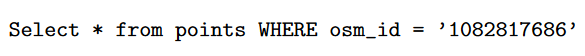
\includegraphics[width=\textwidth]{images/geo_q1.png}
            \caption{Query 1}
        \end{figure}
    \end{minipage}\hfill
    \begin{minipage}{0.43\textwidth}
        \begin{figure}
            \centering
            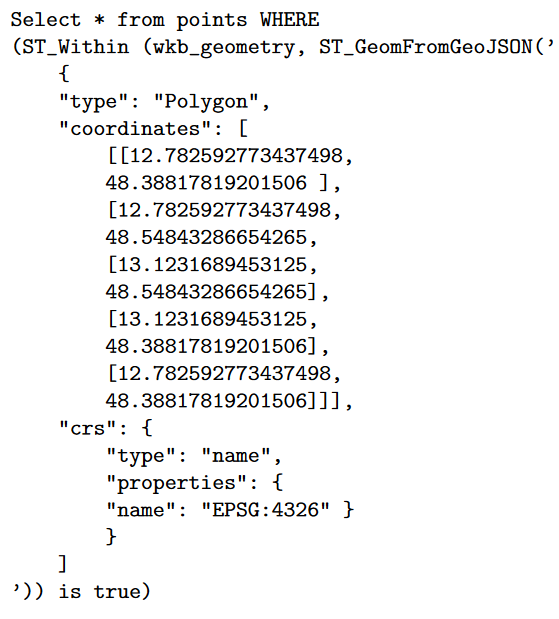
\includegraphics[width=\textwidth]{images/geo_q2.png}
            \caption{Query 2}
        \end{figure}
    \end{minipage}
    
\end{frame}

\begin{frame}
    \frametitle{Performance investigation of selected SQL and NoSQL databases}

    Para realizar la simulación en condiciones realistas, las consultas se realizaron con una determinada cantidad de usuarios, la cuál va en aumento:

    \vspace{-0.4cm}
    
    \begin{center}
        100, 250 y 500 usuarios.
    \end{center}

     

    \begin{minipage}{0.48\textwidth}
        \begin{figure}
            \centering
            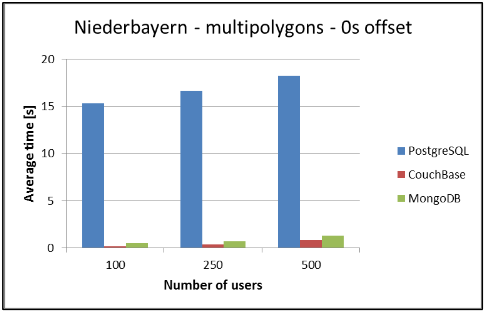
\includegraphics[width=\textwidth]{images/geo-g1.png}
            \caption{Resultados Query 1}
        \end{figure}
    \end{minipage}\hfill
    \begin{minipage}{0.48\textwidth}
        \begin{figure}
            \centering
            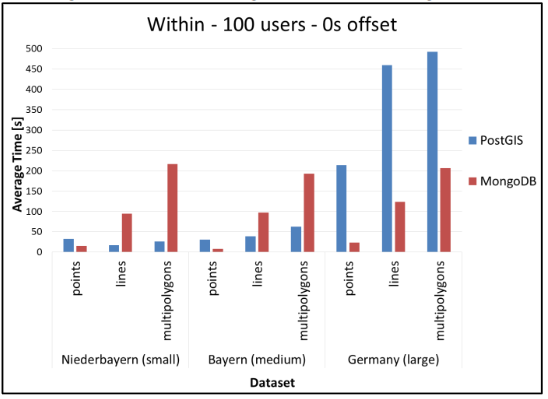
\includegraphics[width=\textwidth]{images/geo-g2.png}
            \caption{Resultados Query 2}
        \end{figure}
    \end{minipage}
\end{frame}

\subsubsection{Conclusiones}

\begin{frame}
    \frametitle{Performance investigation of selected SQL and NoSQL databases - Conclusión}

    \begin{itemize}
        \item Las consultas con el uso de geo-funciones llevan más tiempo que las consultas sobre información de atributos.

         
        
        \item Para solicitudes puramente sobre información de atributos, las bases de datos NoSQL son superiores en comparación con las bases de datos SQL.

         
        
        \item Los resultados muestran claramente que las bases de datos NoSQL son una alternativa posible, al menos para consultar información de atributos.
    \end{itemize}
\end{frame}